\documentclass[11pt,a4paper]{report}

\usepackage[utf8]{inputenc}
\usepackage[T1]{fontenc}
\usepackage{lmodern}
\usepackage{geometry}
\usepackage{amsmath,amssymb,mathtools}
\usepackage{bm}
\usepackage{graphicx}
\usepackage{booktabs}
\usepackage{siunitx}
\usepackage{hyperref}
\usepackage{caption}
\usepackage{subcaption}
\usepackage{float}
\geometry{margin=1in}
\hypersetup{colorlinks=true,linkcolor=blue,citecolor=blue,urlcolor=blue}

\title{Wave Equation FEM Project Report\\
\large Detailed Mathematical Derivation, Method Analysis, and Numerical Evidence}
\author{Qiansong\ Li\ \ Chengxi\ Rao\ \ Chenyu\ Ye\ \ Zhenyu\ Zhao}
\date{\today}

\begin{document}

\maketitle
\pagenumbering{roman}
\tableofcontents
\clearpage
\pagenumbering{arabic}
\setcounter{page}{1}

\chapter{Mathematical Model and Space Discretization}
\section{Strong Form and Initial-Boundary Value Problem}
Let $\Omega\subset\mathbb{R}^2$ be a bounded domain, $T>0$, and consider
\begin{equation}
\begin{cases}
\partial_{tt}u - \Delta u = f & \text{in } \Omega\times(0,T),\\
u = g & \text{on } \partial\Omega\times(0,T),\\
u(\cdot,0)=u_0,\quad \partial_tu(\cdot,0)=v_0 & \text{in } \Omega.
\end{cases}
\label{eq:strong}
\end{equation}
In the code, the main verification setting is an eigenmode with homogeneous boundary ($g=0$), while an additional driven boundary case is also implemented.

\section{Weak Formulation (Homogeneous Dirichlet Case)}
Assume first $g=0$ and define
\[
V:=H_0^1(\Omega)=\{w\in H^1(\Omega):w|_{\partial\Omega}=0\}.
\]
Multiply \eqref{eq:strong} by a test function $v\in V$ and integrate over $\Omega$:
\begin{equation}
\int_\Omega \partial_{tt}u\,v\,dx - \int_\Omega \Delta u\,v\,dx = \int_\Omega f\,v\,dx.
\end{equation}
Use Green's identity on the Laplacian term:
\[
-\int_\Omega \Delta u\,v\,dx = \int_\Omega \nabla u\cdot\nabla v\,dx - \int_{\partial\Omega} \frac{\partial u}{\partial n}v\,ds.
\]
Since $v|_{\partial\Omega}=0$, the boundary term vanishes, hence
\begin{equation}
(\partial_{tt}u,v) + a(u,v) = (f,v),\qquad \forall v\in V,
\label{eq:weak}
\end{equation}
with
\[
a(w,v):=\int_\Omega \nabla w\cdot\nabla v\,dx.
\]

\section{Non-homogeneous Dirichlet Data by Lifting}
For $u=g$ on $\partial\Omega$, introduce a lifting $\tilde g(\cdot,t)\in H^1(\Omega)$ such that $\tilde g|_{\partial\Omega}=g$, and set
\[
u = w+\tilde g,\qquad w\in H_0^1(\Omega).
\]
Substituting into \eqref{eq:weak} gives
\begin{equation}
(\partial_{tt}w,v)+a(w,v)=(f,v) - (\partial_{tt}\tilde g,v)-a(\tilde g,v),\quad \forall v\in V.
\label{eq:lifting}
\end{equation}
This is the mathematically clean way to treat non-homogeneous Dirichlet data. In implementation, we directly enforce boundary DOFs each step (equivalent to lifting at algebraic level).

\section{Finite Element Semi-discretization in Space}
Choose $V_h\subset V$ with basis $\{\phi_i\}_{i=1}^N$ and write
\[
u_h(x,t)=\sum_{j=1}^N U_j(t)\phi_j(x).
\]
Using $v_h=\phi_i$ leads to
\begin{equation}
\sum_{j=1}^N M_{ij}\ddot U_j + \sum_{j=1}^N K_{ij}U_j = F_i,
\end{equation}
with
\begin{equation}
M_{ij}=\int_\Omega \phi_i\phi_j\,dx,\qquad
K_{ij}=\int_\Omega \nabla\phi_i\cdot\nabla\phi_j\,dx,
\qquad
F_i=\int_\Omega f\phi_i\,dx.
\end{equation}
In vector form:
\begin{equation}
M\ddot{\bm U}(t)+K\bm U(t)=\bm F(t).
\label{eq:semi_discrete}
\end{equation}

\chapter{Time Discretization: Mathematical Analysis of Central Difference and Newmark}
\section{Central Difference Method}
\subsection{Derivation}
From \eqref{eq:semi_discrete}, approximate acceleration at $t_n=n\Delta t$ by
\[
\ddot{\bm U}^n\approx \frac{\bm U^{n+1}-2\bm U^n+\bm U^{n-1}}{\Delta t^2}.
\]
For $\bm F=0$, we obtain
\begin{equation}
\bm U^{n+1}=2\bm U^n-\bm U^{n-1}-\Delta t^2 M^{-1}K\bm U^n.
\label{eq:cd_update}
\end{equation}
This is explicit once $M^{-1}$ is cheap (especially with lumped mass).

\subsection{Stability and Dispersion Characteristics}
Let $\lambda_j$ be eigenvalues of $M^{-1}K$. Modal analysis yields a CFL-like condition
\begin{equation}
\Delta t\le \frac{2}{\sqrt{\lambda_{\max}(M^{-1}K)}}.
\label{eq:cfl}
\end{equation}
When \eqref{eq:cfl} is violated, high-frequency modes grow rapidly (numerical blow-up). Even in stable range, phase errors remain (numerical dispersion), more visible on coarse meshes or large $\Delta t/h$.

\section{Newmark-\texorpdfstring{$\beta$}{beta} Method}
Starting from the semi-discrete equation
\[
M\ddot{\bm U}(t)+K\bm U(t)=\bm F(t),
\]
assume that at time $t_n$ we know $(\bm U^n,\bm V^n,\bm A^n)$ with
\[
\bm A^n=M^{-1}(\bm F^n-K\bm U^n).
\]
The Newmark-$\beta$ family introduces the kinematic update formulas
\begin{align}
\bm U^{n+1} &= \bm U^n + \Delta t\,\bm V^n
              + \Delta t^2\!\left(\tfrac12-\beta\right)\bm A^n
              + \beta\Delta t^2\bm A^{n+1}, \label{eq:newmark_disp}\\
\bm V^{n+1} &= \bm V^n + \Delta t(1-\gamma)\bm A^n
              + \gamma\Delta t\,\bm A^{n+1}. \label{eq:newmark_vel}
\end{align}
Equation \eqref{eq:newmark_disp} gives
\[
\bm A^{n+1}
=\frac{1}{\beta\Delta t^2}
\left(\bm U^{n+1}-\bm U^n-\Delta t\,\bm V^n
-\Delta t^2\!\left(\tfrac12-\beta\right)\bm A^n\right).
\]
Define the displacement predictor
\[
\bm U^{\star}
=\bm U^n+\Delta t\,\bm V^n+\Delta t^2\!\left(\tfrac12-\beta\right)\bm A^n,
\]
so that
\[
\bm A^{n+1}=\frac{1}{\beta\Delta t^2}\left(\bm U^{n+1}-\bm U^{\star}\right).
\]
Now enforce equilibrium at $t_{n+1}$:
\[
M\bm A^{n+1}+K\bm U^{n+1}=\bm F^{n+1}.
\]
Substituting $\bm A^{n+1}$ yields
\[
\frac{1}{\beta\Delta t^2}M\left(\bm U^{n+1}-\bm U^\star\right)+K\bm U^{n+1}
=\bm F^{n+1},
\]
which can be rearranged as
\begin{equation}
\left(M+\beta\Delta t^2K\right)\bm U^{n+1}
=M\bm U^\star+\beta\Delta t^2\bm F^{n+1}.
\label{eq:newmark_system}
\end{equation}
This is the linear system solved at each step in the implementation. Once
$\bm U^{n+1}$ is computed, acceleration and velocity are updated by
\begin{align}
\bm A^{n+1} &= \frac{1}{\beta\Delta t^2}\left(\bm U^{n+1}-\bm U^\star\right),\\
\bm V^{n+1} &= \bm V^n + \Delta t(1-\gamma)\bm A^n + \gamma\Delta t\,\bm A^{n+1}.
\end{align}
The central difference method can be viewed as a special explicit member of the
same Newmark family (for specific parameter choices). In this project we use
the average-acceleration choice $(\beta,\gamma)=(1/4,1/2)$, which is
second-order accurate for linear problems and unconditionally stable in the
standard linear setting. It is also nearly non-dissipative in long-time wave
propagation, while choices with $\gamma>1/2$ introduce algorithmic damping of
high-frequency modes. The tradeoff is that \eqref{eq:newmark_system} is
implicit and requires a sparse linear solve per time step. In the code, this
solve is handled by \texttt{SparseDirectUMFPACK} (UMFPACK backend).

\chapter{Mass Matrix Choices: Consistent vs Lumped}
\section{Consistent Mass}
The consistent mass matrix uses the exact FE inner product:
\[
M_{ij}=\int_\Omega\phi_i\phi_j\,dx.
\]
Properties:
\begin{itemize}
  \item symmetric positive definite,
  \item mathematically faithful to Galerkin projection,
  \item generally non-diagonal, so explicit steps require solving/inverting a sparse system.
\end{itemize}

\section{Lumped Mass}
Lumping replaces $M$ by a diagonal approximation (here row-sum lumping):
\[
M^{\text{lump}}_{ii}=\sum_j M_{ij},\qquad M^{\text{lump}}_{ij}=0\ (i\neq j).
\]
Properties:
\begin{itemize}
  \item very cheap explicit updates (component-wise division),
  \item changes the discrete inner product, introducing extra quadrature/modeling error,
  \item often preferred for explicit wave propagation due to efficiency.
\end{itemize}

\section{Practical Implications in This Project}
\subsection{Central Difference + Lumped Mass}
This combination uses
\[
\bm U^{n+1}=2\bm U^n-\bm U^{n-1}-\Delta t^2(M^{\mathrm{lump}})^{-1}K\bm U^n.
\]
Because $M^{\mathrm{lump}}$ is diagonal, $(M^{\mathrm{lump}})^{-1}$ is applied
component-wise, so each step is very cheap. The main limitation is the CFL-type
restriction \eqref{eq:cfl}; if $\Delta t/h$ is too large, high-frequency modes
become unstable quickly.

\subsection{Central Difference + Consistent Mass}
The time update remains explicit in form, but acceleration requires
\[
M\bm A^n=-K\bm U^n
\]
with a sparse linear solve for each step (or each stage where $M^{-1}$ is
applied). This increases cost compared with lumped mass. In return, the mass
representation is closer to the exact Galerkin inner product, which may improve
physical fidelity for some wave metrics.

\subsection{Newmark + Lumped Mass}
Even with diagonal mass, the implicit Newmark system is
\[
\left(M^{\mathrm{lump}}+\beta\Delta t^2K\right)\bm U^{n+1}
=M^{\mathrm{lump}}\bm U^\star+\beta\Delta t^2\bm F^{n+1}.
\]
The stiffness term couples unknowns globally, so a sparse linear solve is still
required at every step. Compared with central difference, this removes the
explicit CFL barrier in the standard linear analysis but increases per-step
algebraic cost.

\subsection{Newmark + Consistent Mass}
This is the fully implicit Galerkin-consistent variant:
\[
\left(M+\beta\Delta t^2K\right)\bm U^{n+1}
=M\bm U^\star+\beta\Delta t^2\bm F^{n+1}.
\]
It combines implicit time integration with consistent mass and is typically the
most robust option among the four for stiff or long-time runs. In this project,
the linear systems for this case are solved with \texttt{SparseDirectUMFPACK}.

\chapter{Numerical Results and Analysis}
\section{Experimental Setup}
Main setup used for comparisons:
\begin{itemize}
  \item domain: unit square simplex meshes,
  \item exact-mode benchmark: $u(x,y,t)=\sin(\pi x)\sin(\pi y)\cos(\omega t)$ with $\omega=\sqrt{2}\pi$,
  \item output data: error CSV and energy CSV,
  \item scripts: batch runner and plot generators from \texttt{scripts/}.
\end{itemize}

\section{Convergence Plots}
\begin{figure}[H]
  \centering
  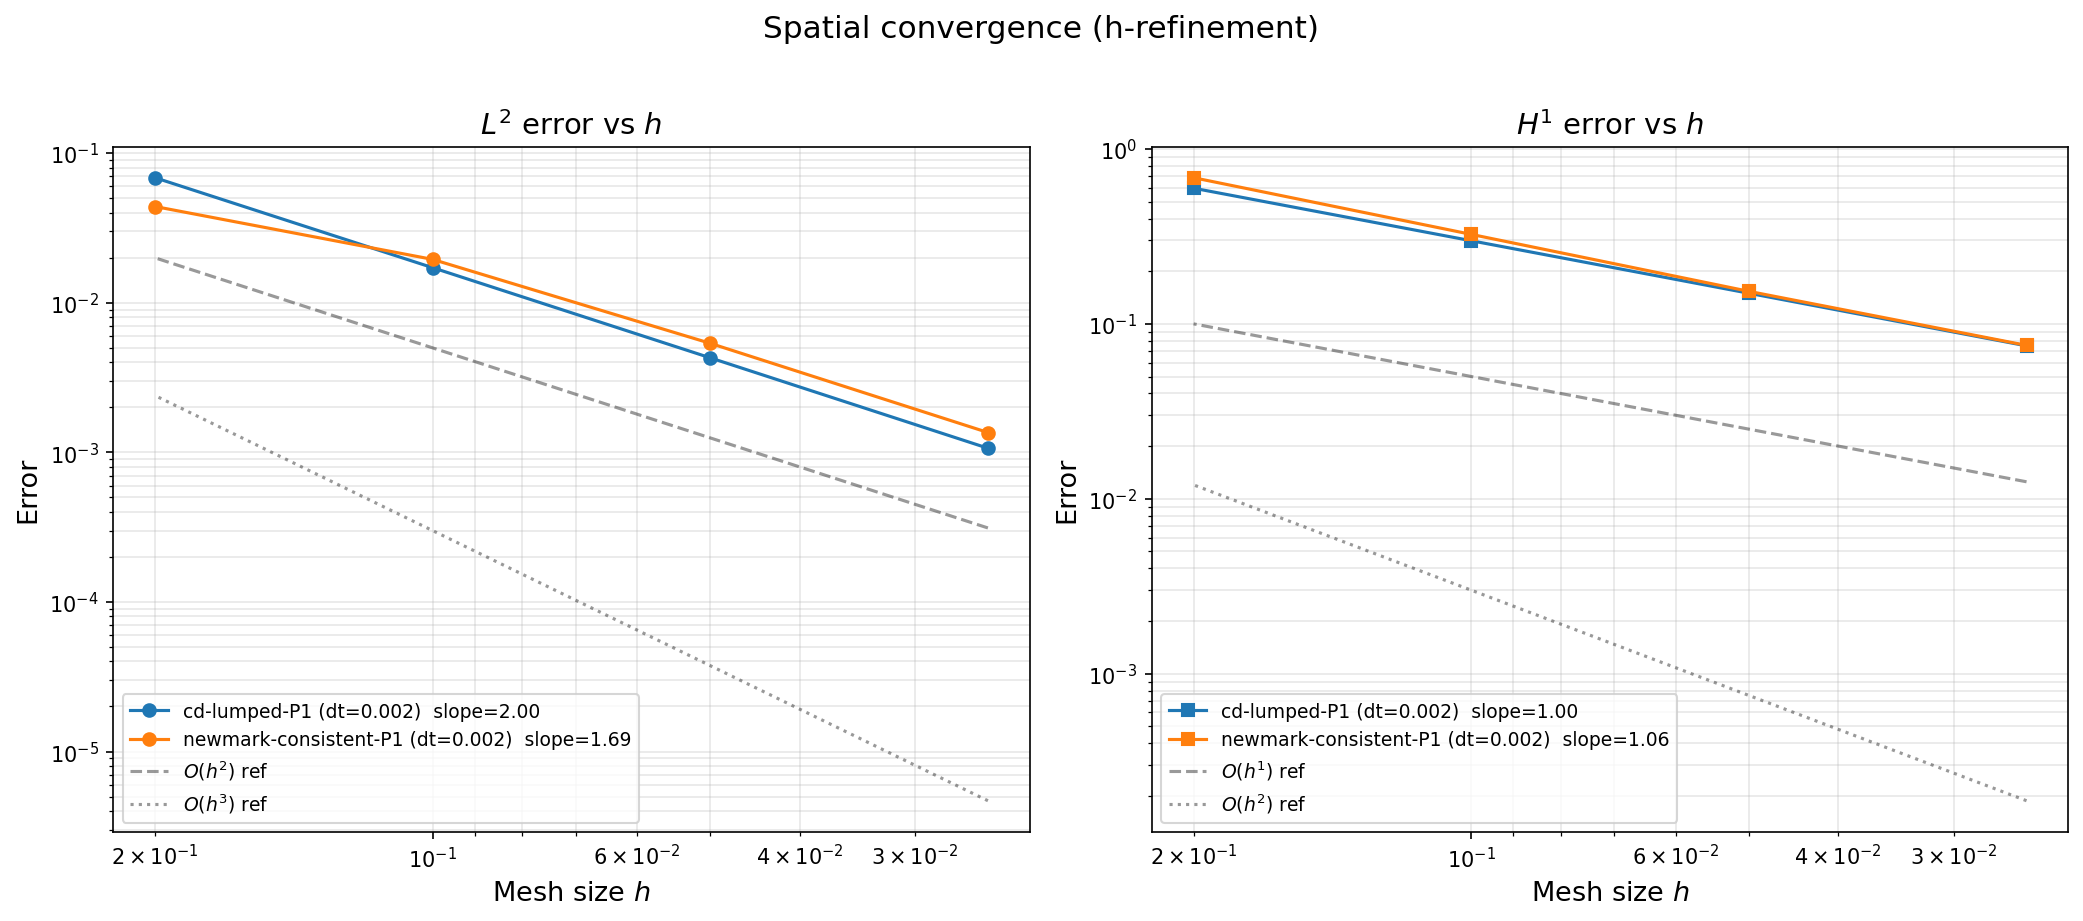
\includegraphics[width=0.82\textwidth]{pic/convergence_h.png}
  \caption{Spatial refinement convergence.}
  \label{fig:conv_h}
\end{figure}

Figure~\ref{fig:conv_h} shows that both norms decrease under mesh refinement.
For linear elements ($p=1$), standard finite-element estimates for smooth
solutions give
\[
\|u-u_h\|_{H^1(\Omega)} \le C h \|u\|_{H^2(\Omega)},
\]
and, by an Aubin--Nitsche duality argument,
\[
\|u-u_h\|_{L^2(\Omega)} \le C h^2 \|u\|_{H^2(\Omega)}.
\]
After adding second-order time discretization (central difference or
Newmark-$\beta$ with $\gamma=\tfrac12$), the fully discrete error is
well described by
\[
\|e\|_{H^1} \lesssim C_1 h + C_2 \Delta t^2,\qquad
\|e\|_{L^2} \lesssim C_3 h^2 + C_4 \Delta t^2.
\]
In the plotted runs, $\Delta t$ is small enough that spatial terms dominate,
so the $L^2$ curves approach second-order behavior, while the $H^1$ curves
approach first-order behavior, consistent with theory.

\begin{figure}[H]
  \centering
  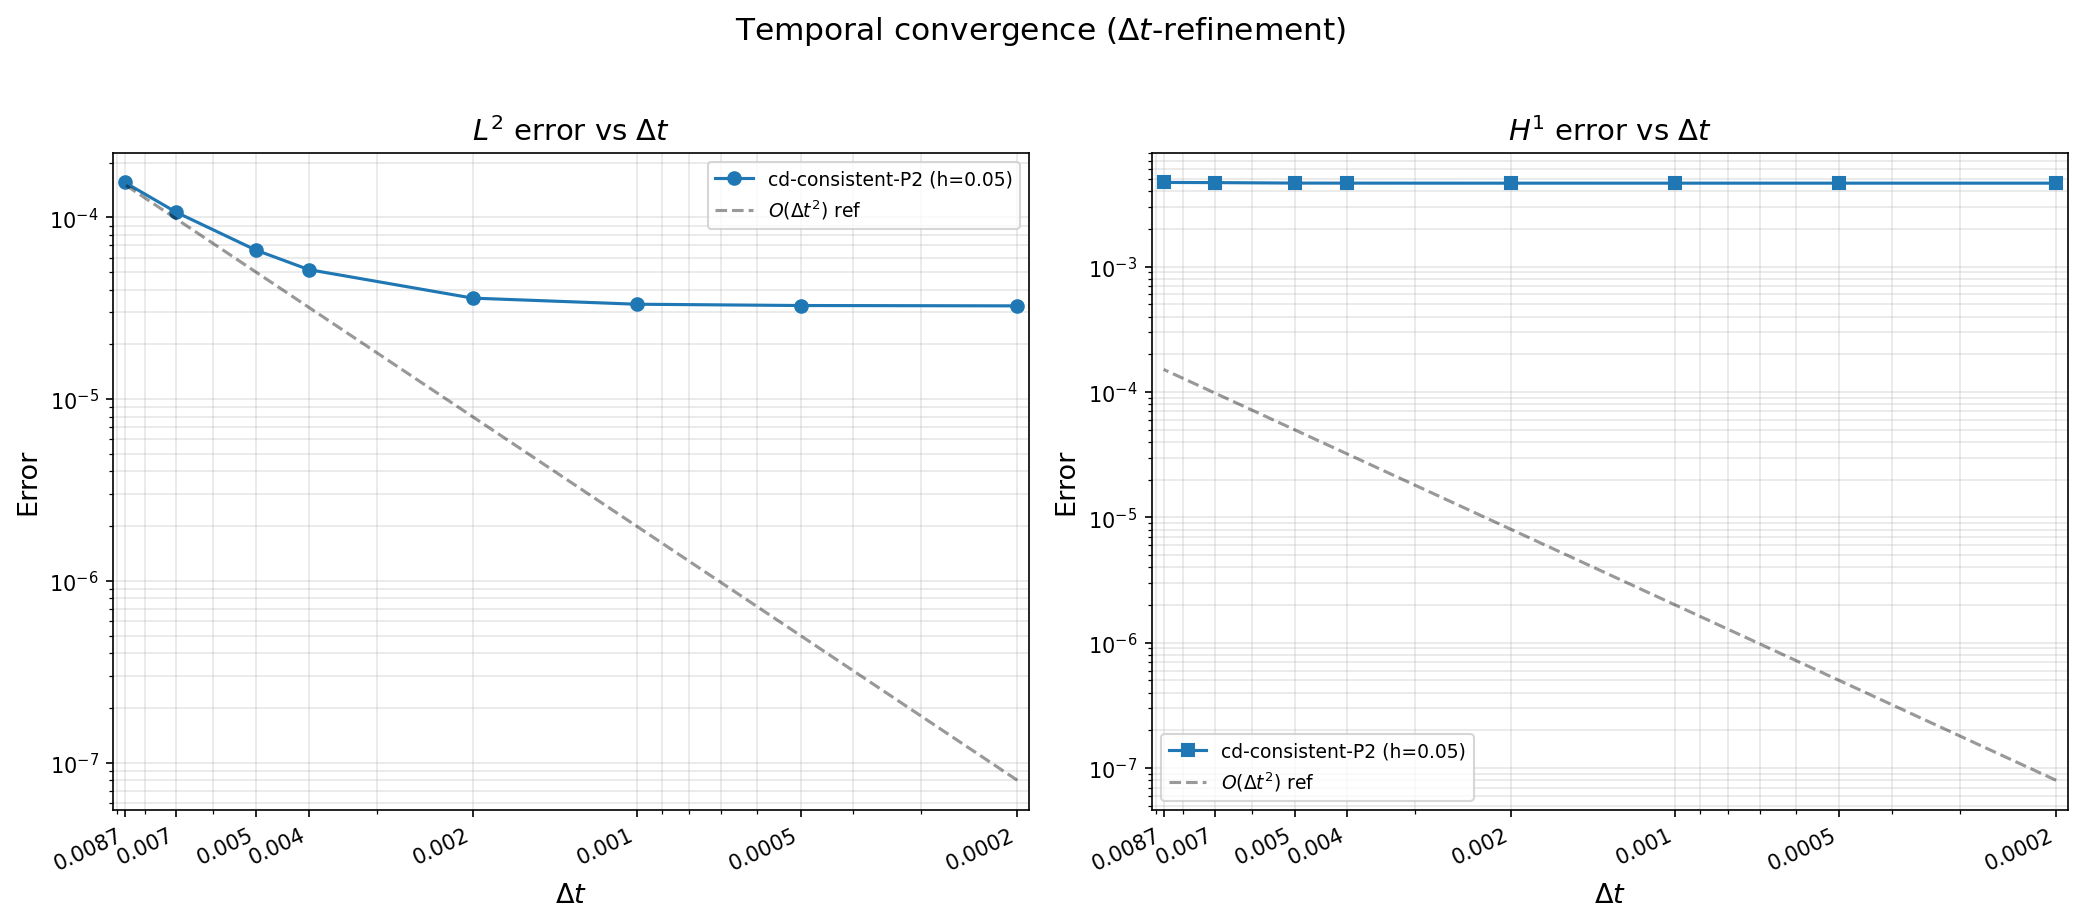
\includegraphics[width=0.82\textwidth]{pic/convergence_dt_cd.png}
  \caption{Temporal refinement convergence for central difference (consistent mass, $P2$, $h=0.05$).}
  \label{fig:conv_dt}
\end{figure}

\begin{figure}[H]
  \centering
  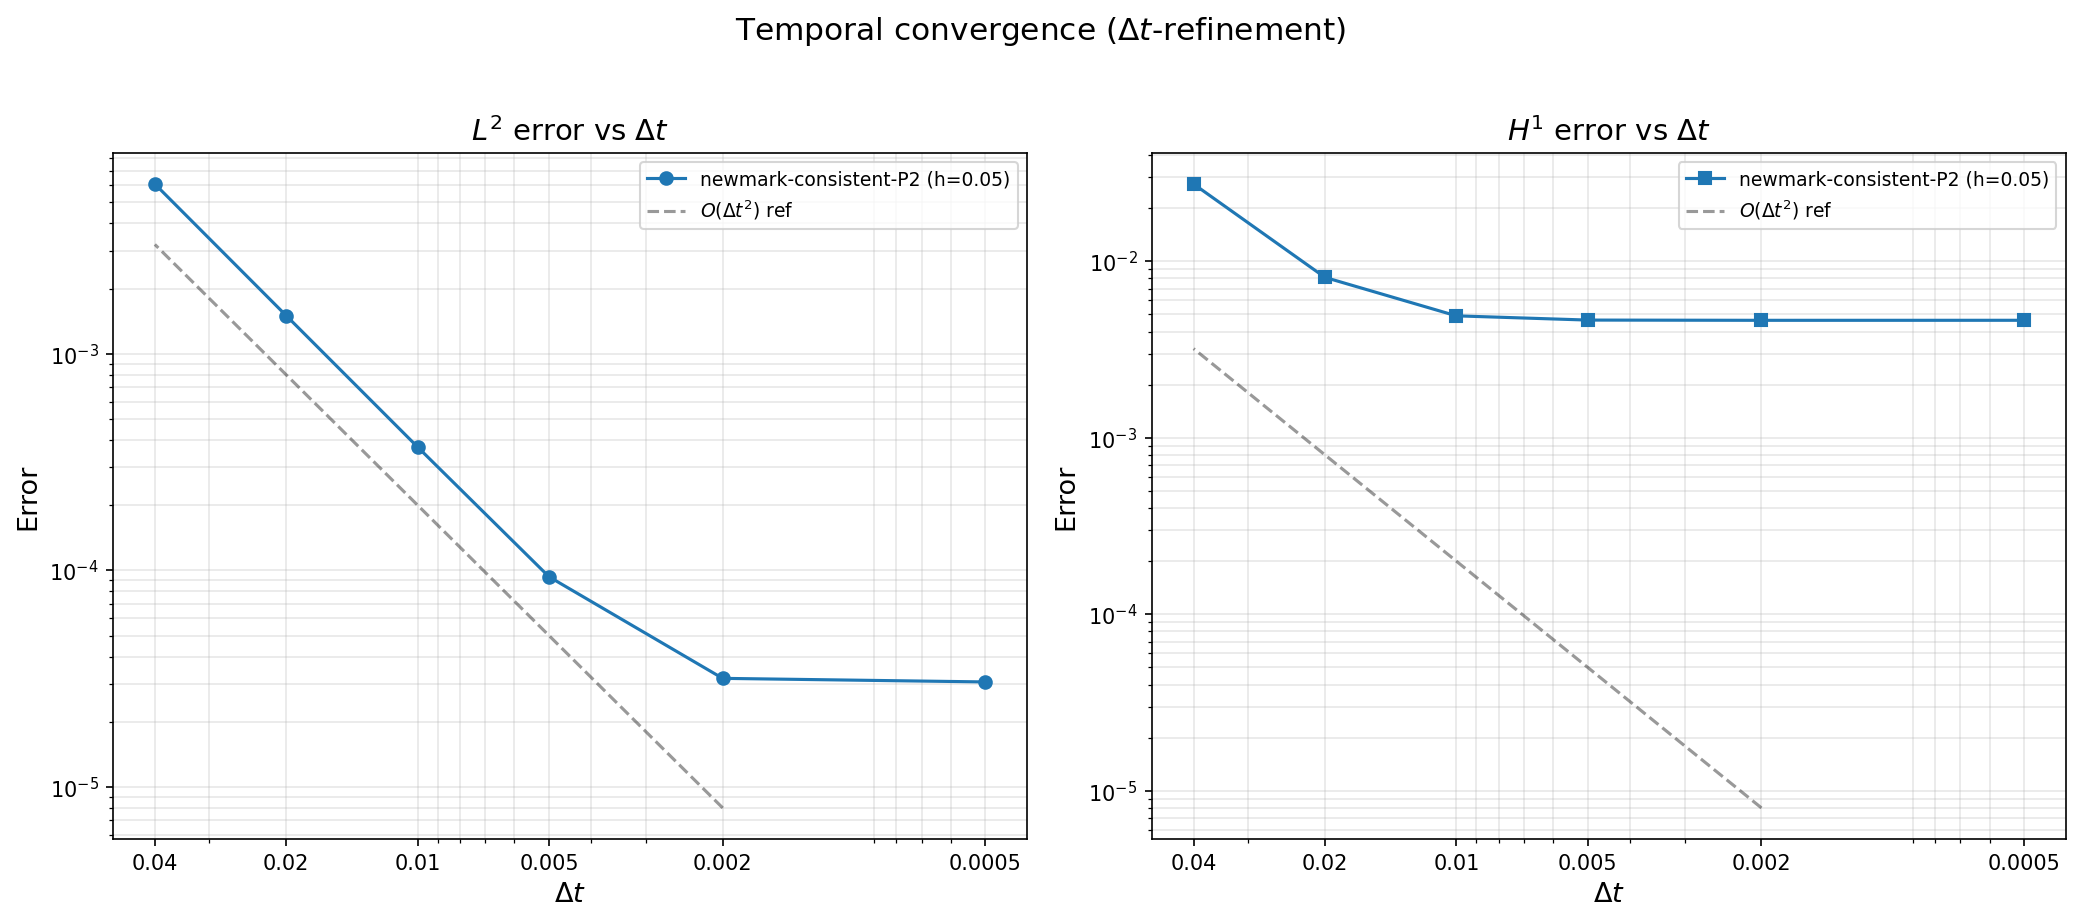
\includegraphics[width=0.82\textwidth]{pic/convergence_dt_newmark.png}
  \caption{Temporal refinement convergence for Newmark (consistent mass, $P2$, $h=0.05$).}
\end{figure}

To interpret Figures~4.2 and~4.3, start from the semi-discrete system
\[
M\ddot{\bm u}(t)+K\bm u(t)=\bm 0.
\]
Let $\bm u^\star(t_n)$ denote the exact solution of this ODE sampled at
$t_n=n\Delta t$, and $\bm u^n$ the fully discrete value.
The total error is split as
\[
\bm u(t_n)-\bm u^n
=\underbrace{\big(\bm u(t_n)-\bm u^\star(t_n)\big)}_{\text{space error}}
+\underbrace{\big(\bm u^\star(t_n)-\bm u^n\big)}_{\text{time error}}.
\]

For central difference,
\[
\frac{\bm u^{n+1}-2\bm u^n+\bm u^{n-1}}{\Delta t^2}
=\ddot{\bm u}(t_n)+\mathcal O(\Delta t^2),
\]
so the local truncation defect is second order. Under the CFL stability bound,
the global time error is therefore
\[
\|\bm u^\star(t_n)-\bm u^n\|\le C_T\,\Delta t^2.
\]
For Newmark with $(\beta,\gamma)=(1/4,1/2)$ (trapezoidal rule),
Taylor expansion of the update pair also gives a second-order consistent method,
and the global bound has the same order:
\[
\|\bm u^\star(t_n)-\bm u^n\|\le \widetilde C_T\,\Delta t^2.
\]

Combining with the spatial estimates for smooth solutions,
\[
\|\bm u-\bm u_h\|_{L^2}\le C_S h^{p+1},\qquad
\|\bm u-\bm u_h\|_{H^1}\le C_S' h^p,
\]
we obtain, at fixed $h$,
\[
\|e^n\|_{L^2}\lesssim C_S h^{p+1}+C_T\Delta t^2,\qquad
\|e^n\|_{H^1}\lesssim C_S' h^{p}+C_T'\Delta t^2.
\]
Hence, for large-to-moderate $\Delta t$, the $\Delta t^2$ term dominates and
the curves decrease with temporal refinement; once
\[
\Delta t \lesssim \Delta t_\star
\sim \sqrt{\frac{C_S}{C_T}}\,h^{(p+1)/2}
\quad (L^2),\qquad
\Delta t \lesssim \sqrt{\frac{C_S'}{C_T'}}\,h^{p/2}
\quad (H^1),
\]
the spatial term dominates and the curves flatten. This is exactly the
``drop then plateau'' pattern seen in Figures~4.2 and~4.3. The difference
between the two figures is mainly the stability/dispersion constant in front of
the $\Delta t^2$ term: central difference is explicit and CFL-restricted,
whereas Newmark $(1/4,1/2)$ is implicit and not subject to the same explicit
stability cutoff.

\section{Dispersion and Dissipation Diagnostics}
\begin{figure}[H]
  \centering
  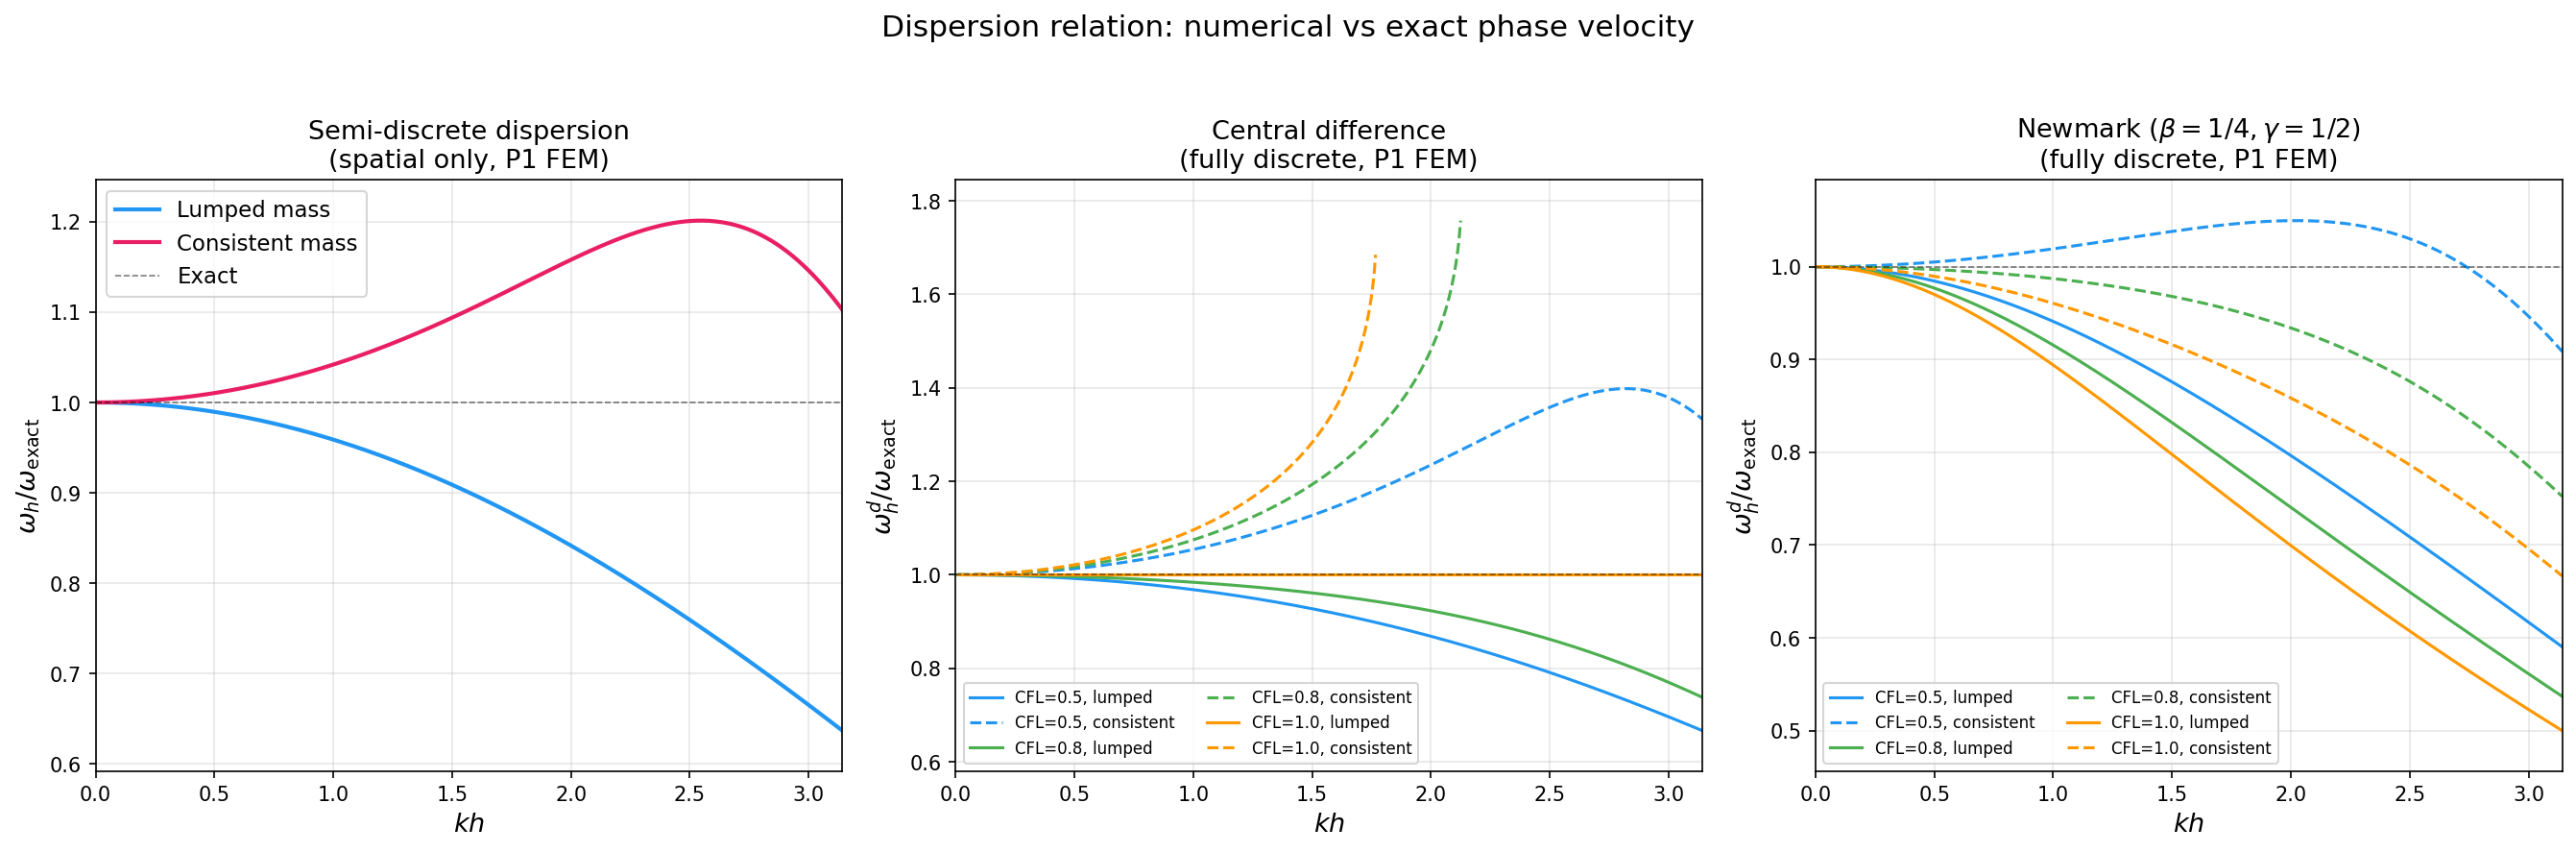
\includegraphics[width=0.82\textwidth]{pic/dispersion_relation.png}
  \caption{Dispersion relation diagnostic (phase-velocity error).}
\end{figure}

\begin{figure}[H]
  \centering
  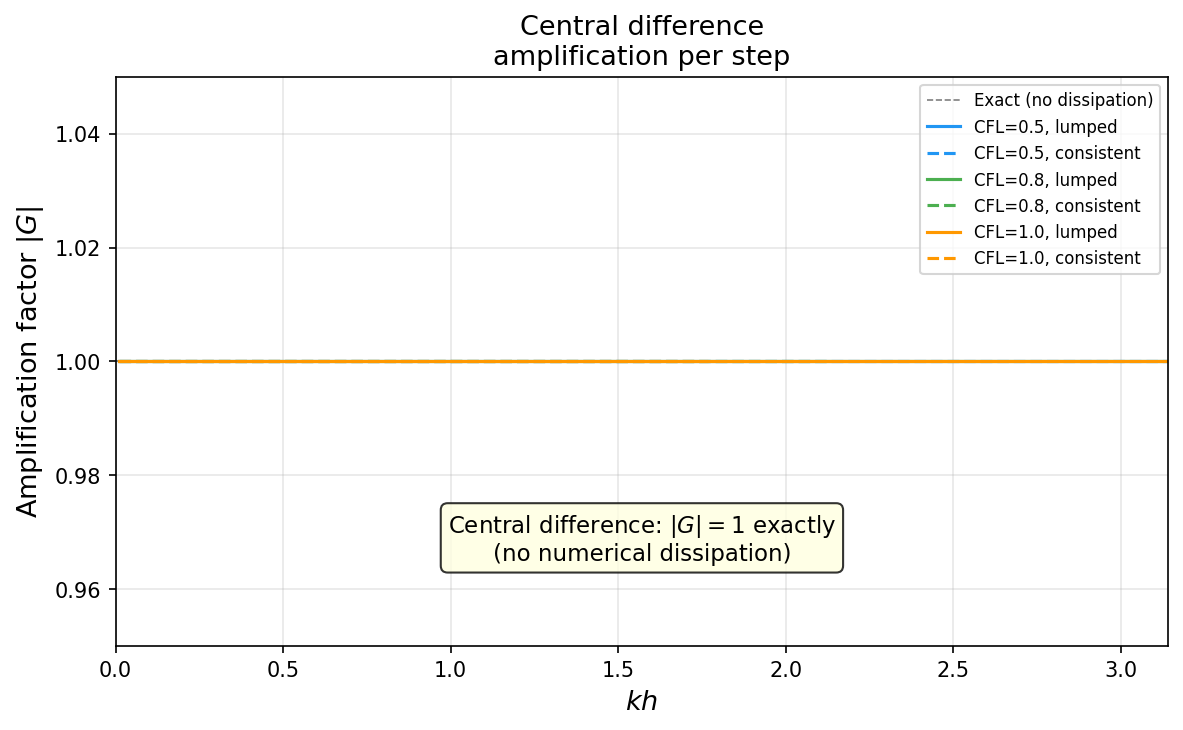
\includegraphics[width=0.75\textwidth]{pic/dissipation_amplification_central.png}
  \caption{Amplification-factor diagnostic for the central difference method.}
\end{figure}

\begin{figure}[H]
  \centering
  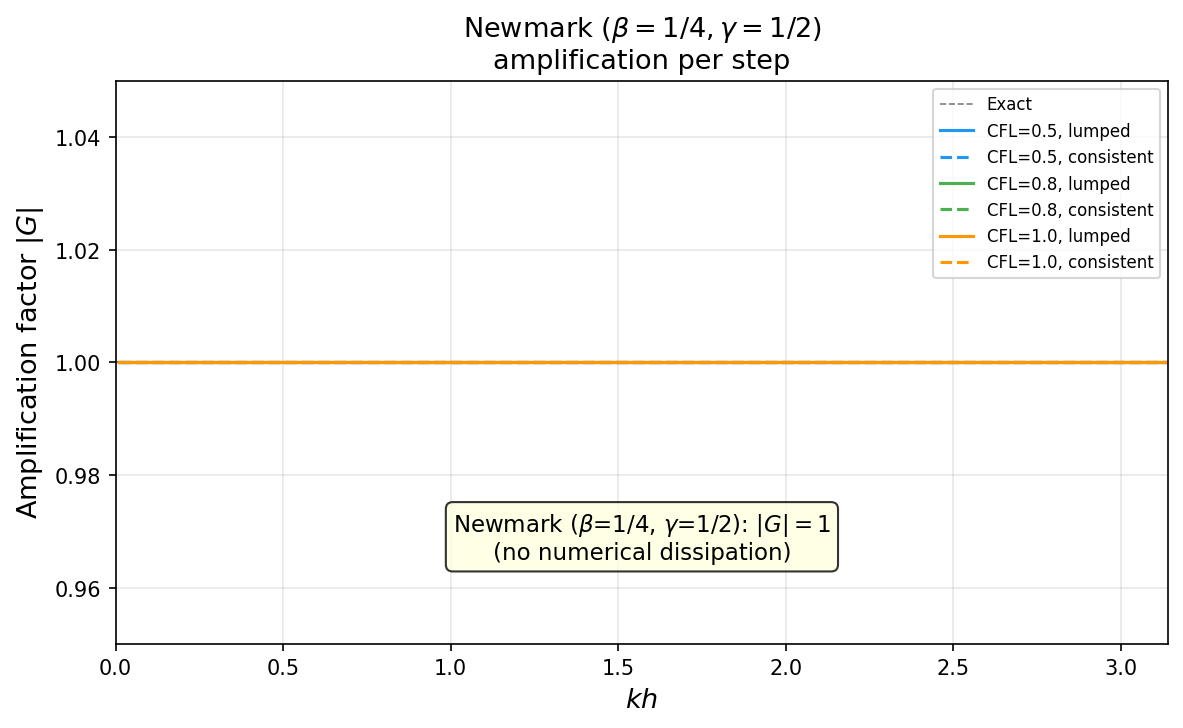
\includegraphics[width=0.75\textwidth]{pic/dissipation_amplification_newmark.png}
  \caption{Amplification-factor diagnostic for Newmark $(\beta,\gamma)=(1/4,1/2)$.}
\end{figure}

Figure~4.4 is based on standard Fourier analysis for 1D P1 FEM on a uniform
mesh (used as a diagnostic proxy for the 2D behavior). With $\xi=kh$,
\[
\lambda_K(\xi)=2(1-\cos\xi),\qquad
\lambda_M^{\rm L}=1,\qquad
\lambda_M^{\rm C}=\frac{2+\cos\xi}{3}.
\]
Hence the semi-discrete frequency satisfies
\[
\omega_h^2(\xi)=\frac{\lambda_K(\xi)}{\lambda_M(\xi)},\qquad
\frac{\omega_h}{\omega_{\rm exact}}=\frac{\sqrt{\lambda_K/\lambda_M}}{\xi},
\]
with $\omega_{\rm exact}=\xi/h$.
This explains the left panel: with lumped mass,
$\lambda_M^{\rm L}$ is constant and $\omega_h/\omega_{\rm exact}<1$ at high
wavenumber (numerical waves are too slow), while with consistent mass,
$\lambda_M^{\rm C}$ decreases as $\xi\to\pi$, so $\omega_h/\omega_{\rm exact}$
can exceed $1$ (high-frequency waves become too fast).

For central difference, the fully discrete dispersion relation is
\[
\cos(\omega_h^d\Delta t)
=1-\frac{\Delta t^2}{2}\,\omega_h^2(\xi).
\]
Using $\Delta t=\nu h$ (CFL number $\nu$), one gets
\[
\omega_h^d h
=\frac{1}{\nu}\arccos\!\left(1-\frac{\nu^2}{2}\omega_h^2(\xi)\right),
\qquad
\frac{\omega_h^d}{\omega_{\rm exact}}
=\frac{\omega_h^d h}{\xi}.
\]
This gives the middle panel behavior: when the argument of $\arccos$ approaches
$-1$, the mapping becomes strongly nonlinear and the ratio bends sharply; once
$|1-\frac{\nu^2}{2}\omega_h^2|>1$, real $\omega_h^d$ no longer exists
(explicit instability cutoff), so high-$\xi$ branches terminate for larger CFL.

For Newmark with $(\beta,\gamma)=(1/4,1/2)$,
\[
\cos(\omega_h^d\Delta t)
=\frac{2-\frac{1}{2}\Delta t^2\omega_h^2(\xi)}
       {2+\frac{1}{2}\Delta t^2\omega_h^2(\xi)}.
\]
The denominator regularizes the high-frequency response, so the right panel
shows smooth curves over the full $\xi$ range and no explicit-cutoff branch
termination, but phase error still grows with $\xi$ (dispersion remains).

In both methods, amplification factors satisfy $|G|\approx 1$ for the
conservative parameter choice used here, so the main mechanism visible in
Figure~4.4 is phase error (dispersion), not artificial damping.

\section{Scheme Comparison on the Same Mesh and Time Step}
\begin{figure}[H]
  \centering
  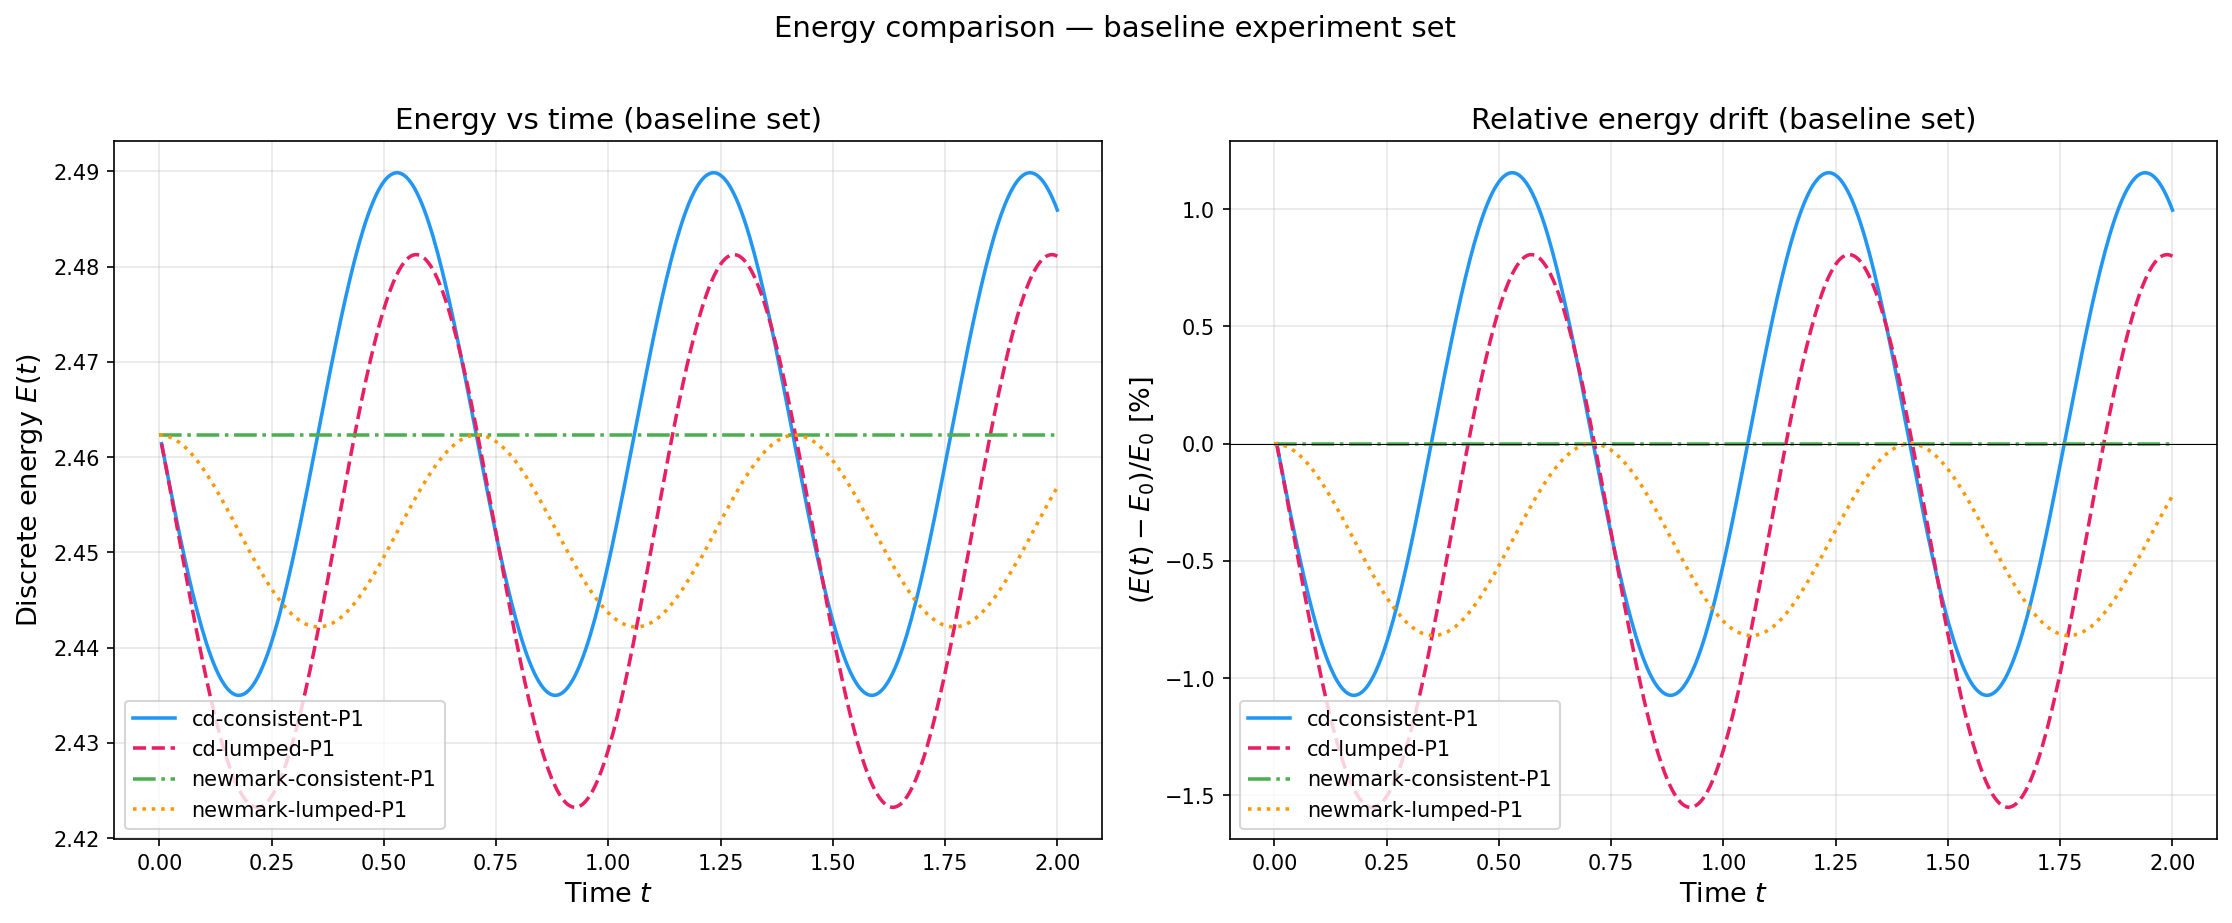
\includegraphics[width=0.9\textwidth]{pic/energy_comparison_baseline.png}
  \caption{Energy comparison across central difference/Newmark and mass variants.}
  \label{fig:energy_cmp}
\end{figure}

The energy comparison uses the drift observable
\[
\delta_E(t)=\frac{E(t)-E_0}{E_0},
\]
with
\[
E(t)=\tfrac12\,\bm v^\top M\bm v+\tfrac12\,\bm u^\top K\bm u.
\]
Different method/mass combinations produce different oscillation envelopes and drift levels. This is expected because the discrete Hamiltonian structure depends jointly on the time integrator and mass representation; phase error and finite-resolution effects modulate how that discrete energy is tracked in long-time simulations.

\begin{figure}[H]
  \centering
  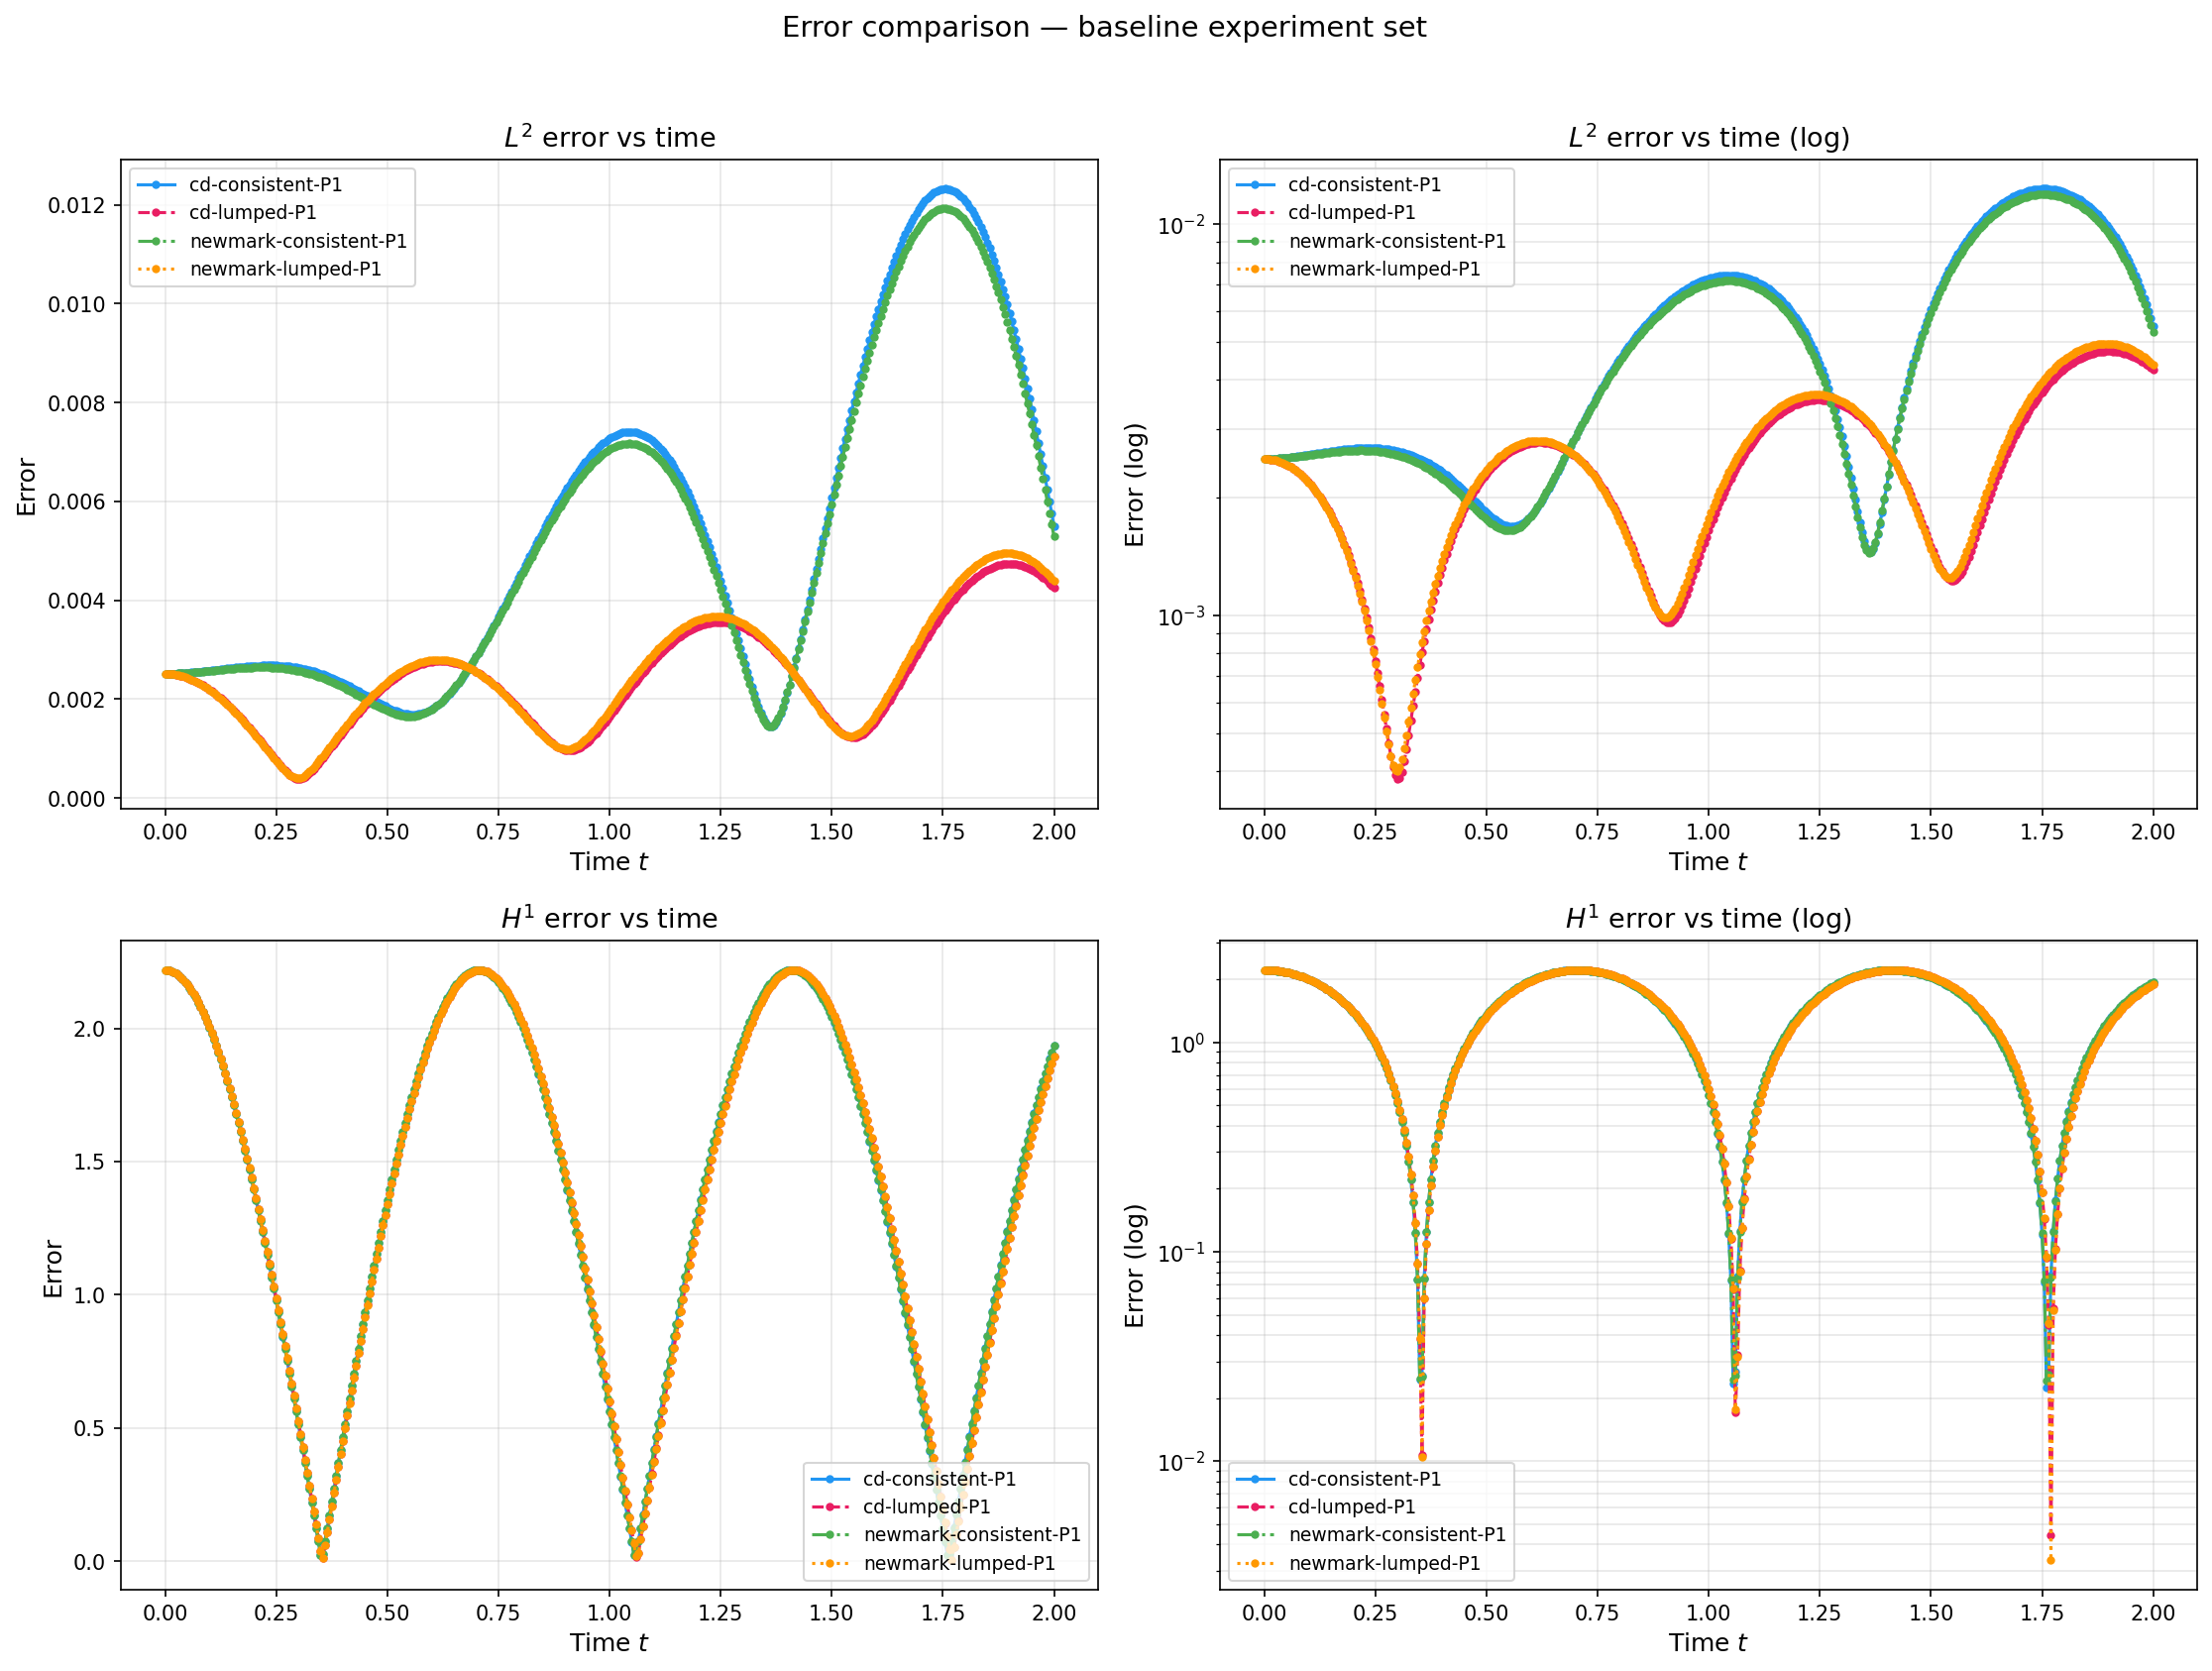
\includegraphics[width=0.9\textwidth]{pic/error_comparison_baseline.png}
  \caption{Error evolution comparison (dispersion-oriented evidence).}
  \label{fig:error_cmp}
\end{figure}

For the same mesh and time step, error trajectories separate over time because the phase mismatch accumulates approximately linearly with the number of steps:
\[
\Delta\phi(t)\approx (\omega_h^d-\omega_{\text{exact}})\,t.
\]
As $\Delta\phi$ grows, pointwise cancellation degrades and both $L^2$ and $H^1$ errors increase at method-dependent rates.

\section{Runtime Comparison Across Time and Mass Combinations}
We benchmarked all four combinations
(central difference/Newmark crossed with lumped/consistent) on the same setup
($h=0.05$, $\Delta t=0.005$, $T=2$, P1, homogeneous boundary). Each case was run five times and we report both mean and median time-stepping wall time, since occasional load spikes can affect single runs.

\begin{table}[H]
  \centering
  \caption{Measured time-stepping cost across time integrator and mass choices.}
  \begin{tabular}{@{}llcccc@{}}
    \toprule
    Time method & Mass type & mean [s] & std [s] & median [s] & relative to fastest \\
    \midrule
    central difference & lumped     & 0.015371 & 0.018418 & 0.008313 & 1.00x \\
    central difference & consistent & 0.052315 & 0.005059 & 0.054807 & 6.59x \\
    Newmark            & lumped     & 0.046572 & 0.009490 & 0.043131 & 5.19x \\
    Newmark            & consistent & 0.053046 & 0.007498 & 0.054282 & 6.53x \\
    \bottomrule
  \end{tabular}
\end{table}

These data support all three points of Section 3.3. First, the central difference method with lumped mass is clearly the fastest configuration. Second, switching central difference from lumped to consistent mass raises cost substantially because each explicit update needs a sparse solve for applying $M^{-1}$. Third, the two Newmark rows are both expensive and close to each other, consistent with the fact that Newmark is implicit and performs a linear solve each time step regardless of mass type.

\section{Supplement A: Newmark Parameter Effect}
\begin{figure}[H]
  \centering
  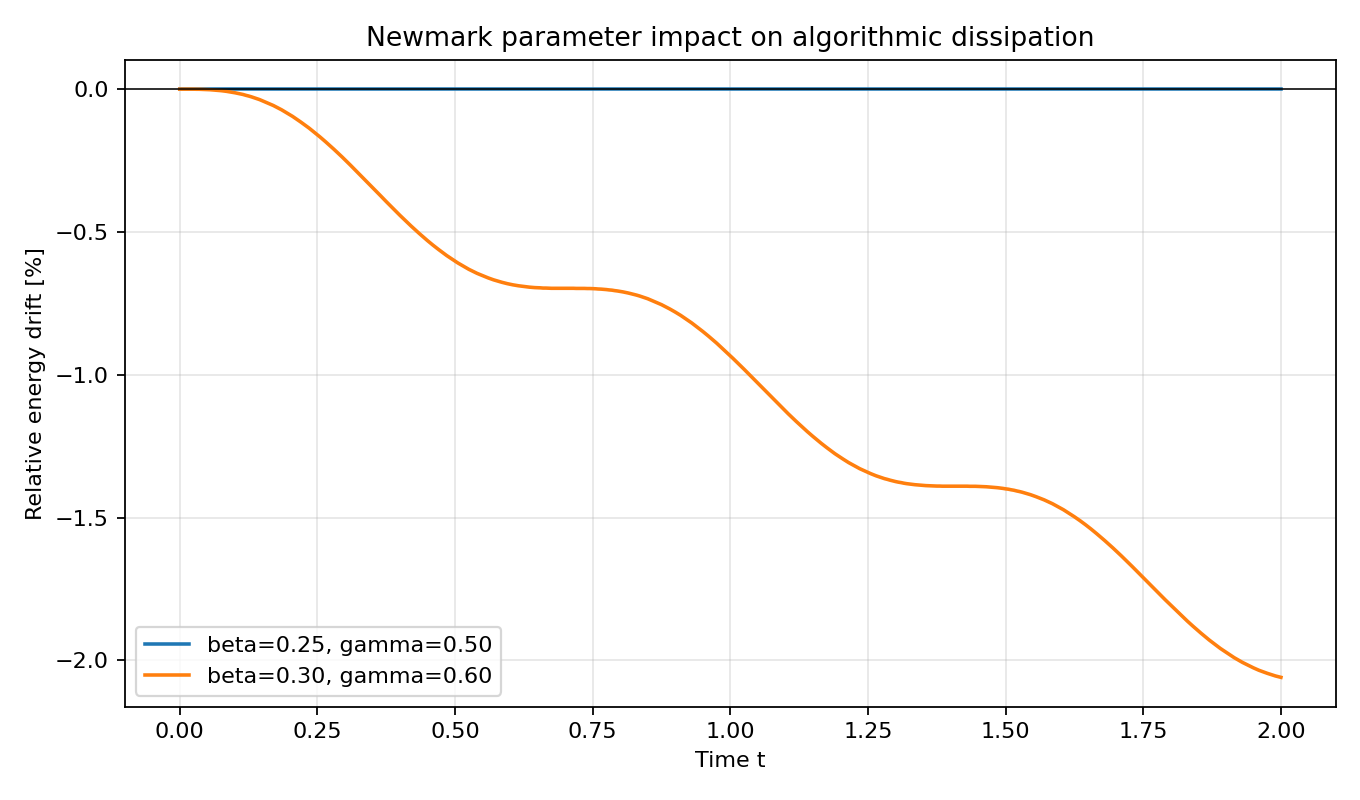
\includegraphics[width=0.78\textwidth]{pic/supplement_newmark_dissipation.png}
  \caption{Relative energy drift for two Newmark parameter sets.}
\end{figure}

The run with $(\beta,\gamma)=(0.3,0.6)$ shows stronger energy decay/drift than $(0.25,0.5)$. This is the expected algorithmic effect of choosing $\gamma>1/2$: the amplification factor for high-frequency components is pushed below one, so those modes are damped numerically and the method departs from near-conservative behavior.

\section{Supplement B: Driven Boundary Energy Injection}
\begin{figure}[H]
  \centering
  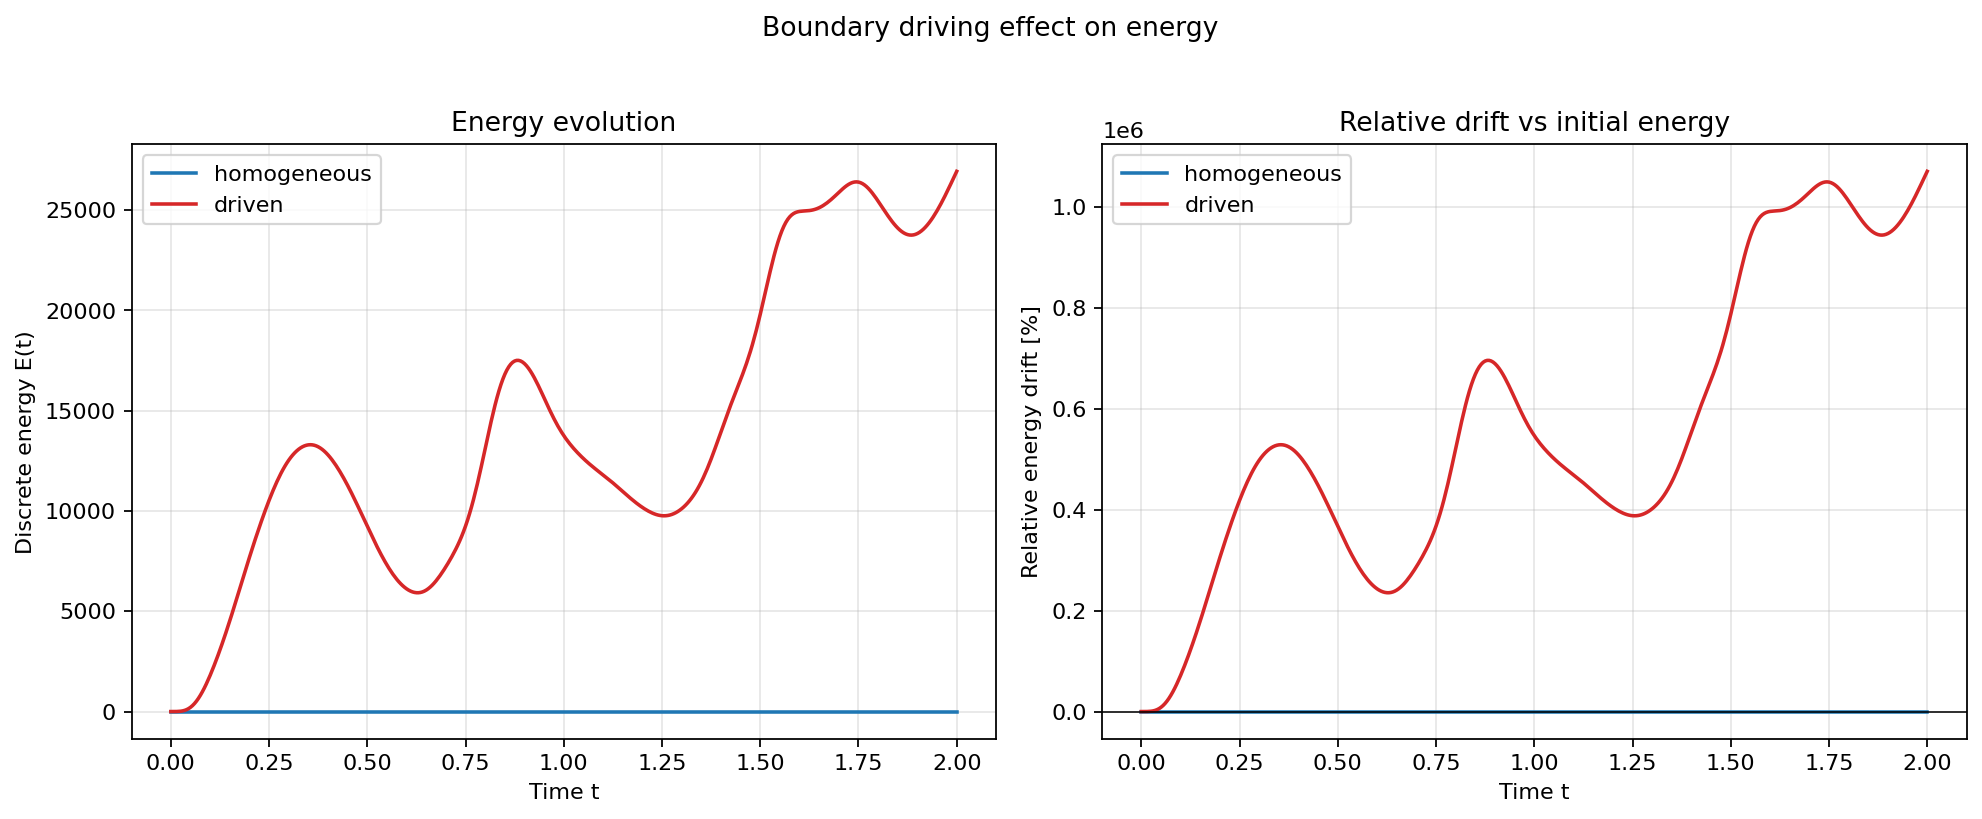
\includegraphics[width=0.9\textwidth]{pic/supplement_boundary_energy.png}
  \caption{Homogeneous vs driven boundary energy diagnostics.}
\end{figure}

Compared to the homogeneous case, the driven-boundary run exhibits strong energy growth. This is consistent with the continuous energy balance
\[
\frac{dE}{dt}=\int_{\partial\Omega}\partial_t u\,\partial_n u\,ds
\]
when boundary motion is imposed. Since the boundary flux is non-zero, energy injection is physical and should not be interpreted as numerical instability by itself.

\section{Supplement C: Explicit CFL Scan}
\begin{figure}[H]
  \centering
  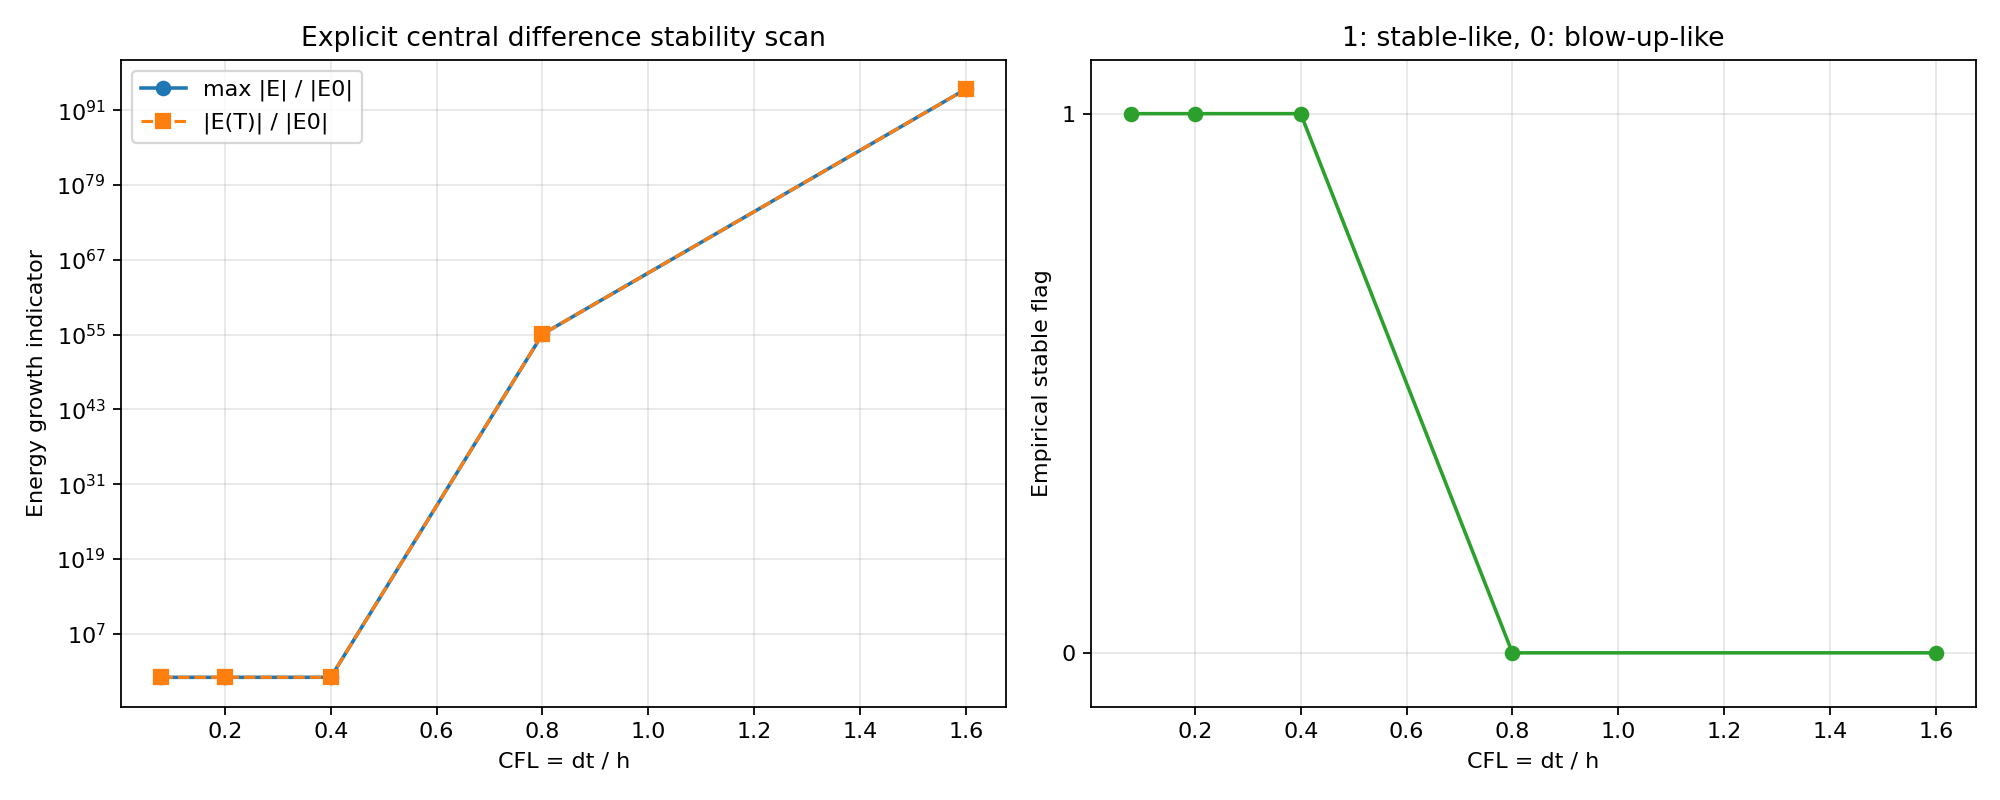
\includegraphics[width=0.85\textwidth]{pic/supplement_cfl_scan.png}
  \caption{Central difference + lumped stability indicator when varying $\Delta t/h$.}
\end{figure}

The CFL scan shows bounded energy for small $\Delta t/h$, followed by explosive growth after a threshold. This matches the modal condition for explicit second-order schemes: stability requires
\[
|G_j|\le 1\quad\forall j,
\]
and once the worst mode violates this bound, high-frequency components are exponentially amplified, producing blow-up in both energy and error norms.

\chapter{Conclusions}
\begin{itemize}
  \item The first-principles derivation from strong form to FE matrix ODE is consistent with implementation.
  \item The central difference method is efficient but CFL-limited; Newmark is robust and parameter-tunable.
  \item Consistent mass is mathematically faithful; lumped mass is computationally attractive for explicit updates.
  \item Figures confirm expected phenomena: near-second-order convergence in baseline cases, dispersion-dominated differences between schemes, controllable Newmark dissipation, physical energy injection under driven boundary, and explicit blow-up past CFL limits.
\end{itemize}

\end{document}
